% !TEX TS-program = pdflatex
% !TEX encoding = UTF-8 Unicode

% This is a simple template for a LaTeX document using the "article" class.
% See "book", "report", "letter" for other types of document.

\documentclass[11pt]{book} % use larger type; default would be 10pt

\usepackage[utf8]{inputenc} % set input encoding (not needed with XeLaTeX)

%%% Examples of Article customizations
% These packages are optional, depending whether you want the features they provide.
% See the LaTeX Companion or other references for full information.

%%% PAGE DIMENSIONS
%\usepackage{geometry} % to change the page dimensions
\usepackage[top=25truemm,bottom=20truemm,left=20truemm,right=20truemm]{geometry}
\geometry{a4paper} % or letterpaper (US) or a5paper or....
% \geometry{margins=2in} % for example, change the margins to 2 inches all round
% \geometry{landscape} % set up the page for landscape
%   read geometry.pdf for detailed page layout information

\usepackage{graphicx} % support the \includegraphics command and options

% \usepackage[parfill]{parskip} % Activate to begin paragraphs with an empty line rather than an indent

%%% PACKAGES
\usepackage{booktabs} % for much better looking tables
\usepackage{array} % for better arrays (eg matrices) in maths
\usepackage{paralist} % very flexible & customisable lists (eg. enumerate/itemize, etc.)
\usepackage{verbatim} % adds environment for commenting out blocks of text & for better verbatim
\usepackage{subfig} % make it possible to include more than one captioned figure/table in a single float
% These packages are all incorporated in the memoir class to one degree or another...
\usepackage{amsmath,amssymb}
\usepackage{framed}
\usepackage{braket}

%%% HEADERS & FOOTERS
\usepackage{fancyhdr} % This should be set AFTER setting up the page geometry
\pagestyle{fancy} % options: empty , plain , fancy
\renewcommand{\headrulewidth}{0pt} % customise the layout...
\lhead{}\chead{}\rhead{}
\lfoot{}\cfoot{\thepage}\rfoot{}

%%% SECTION TITLE APPEARANCE
\usepackage{sectsty}
\allsectionsfont{\sffamily\mdseries\upshape} % (See the fntguide.pdf for font help)
% (This matches ConTeXt defaults)

%%% ToC (table of contents) APPEARANCE
\usepackage[nottoc,notlof,notlot]{tocbibind} % Put the bibliography in the ToC
\usepackage[titles,subfigure]{tocloft} % Alter the style of the Table of Contents
\renewcommand{\cftsecfont}{\rmfamily\mdseries\upshape}
\renewcommand{\cftsecpagefont}{\rmfamily\mdseries\upshape} % No bold!

%%% END Article customizations

%%% The "real" document content comes below...

\title{Thesis}
\author{Fang Ni}
%\date{} % Activate to display a given date or no date (if empty),
         % otherwise the current date is printed 

\begin{document}
\maketitle

\tableofcontents

\chapter{Introduction}

\section{Pairing interaction in nuclei}

Pairing correlation plays an important role near the Fermi energy. Pairing correlation is the two-body interaction which couples two identical nucleons into $J^{\pi}=0^+$ state. There are many evidences of pairing correlation detected from experiment. The most clear evidence is shown in Fig. \ref{Sn_isotope}. All of the ground states of even-even Sn isotopes are $J^{\pi}=0^+$ states  It indicates that the ground states consist of the $J^{\pi}=0^+$ pairs is more stable than other configurations. In addition, the ground states between even-even nuclei and neighborhood odd nuclei has large gaps of binding energy. In odd nuclei, the unpaired last neutron is the last single-particle level. The odd-even mass difference  To break the $J^{\pi}=0^+$ pair, we need large energy which is about $2\Delta \approx 24A^{-1/2}$ MeV.
\begin{figure}[htbp]
 \begin{center}
    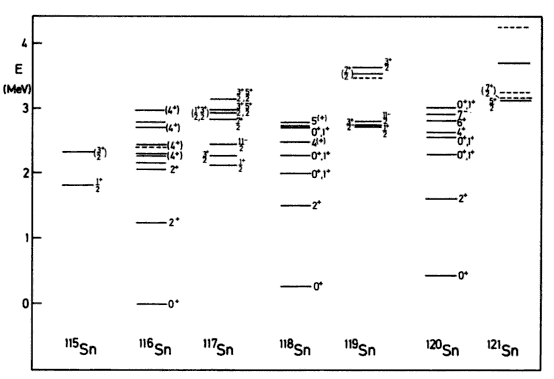
\includegraphics[width=100mm, bb=0 0 400 300]{images/Sn_isotope.png}
 \end{center}
  \caption{Low-lying excited states in Sn isotopes \cite{}. The absolute values of binding energy are adjusted at 0 MeV in the ground state of ${}^{116}$Sn.}
  \label{Sn_isotope}
\end{figure}

\subsection{A subsection}

More text.

\chapter{Pairing model}

To examine the pairing dynamics influencing the structure of nuclei, we can only concentrate the nucleons near the Fermi energy. The Hamiltonian of pairing model is
\begin{align}
	H &= \sum_{l=1}^L \epsilon_l n_l - g \sum_{l,l'} S_l^+ S_{l'}^- ,
\end{align}
where
\begin{align}
	n_l &= \sum_m a^{\dag}_{lm}a_{lm} \\
        S_l^{+} &= \sum_{m>0}a_{lm}^{\dag}a_{l\overline{m}}^{\dag} ,
\quad   S_l^{-} = S_l^{+\dag} .
\label{S_+}
\end{align}
In $L$ single-particle level system, each single-particle energy $\epsilon_l$ possesses $(2\Omega_l)$-fold
degeneracy ($\Omega_l=j_l+1/2$)
and $\sum_{m>0}$ indicates the summation over $m=1/2,3/2,\cdots,$ and $\Omega_l-1/2$. $\overline{m}$ indicates the time reversal quantum number with respect to $m$. The strength of pairing correlation is represented by coupling constant $g$. We also define a seniority $\nu_l$, which is the number of unpaired particles in each level. The unpaired particles have no pairing interaction, and play a part in Pauli blocking effect.\par
In one-level system ($L=1$), the pairing dynamics is well understood. The analytic solution of the total energy is
\begin{align}
	E_{\nu}(N) = \epsilon N - \frac{1}{4}g(N-\nu)(2\Omega-N-\nu+2) .
\end{align}
The pairing rotational band created by the pairing correlation is completely parabolic with the moment of inertia $2/g$. Also, the excited states in a specified $N$ is only described by the quantum number $\nu$. For example, the first excited state in even particle system is $\nu=2$ state, which correspond to one $J^{\pi}=0^+$ pair broken state.\par
The profound dynamics occurs in multi-level pairing model ($L\ge 2$). The pairing rotational mode becomes complex due to the shell effect. In addition, several pairing vibrational modes emerge. The pairing vibration is not single particle motion specified by $\nu_l$, but a collective motion with the excitation of $J^{\pi}=0^+$ pairs. In this chapter, we explain the numerical exact solution and derive the TDHFB dynamics in multi-level pairing Hamiltonian.

\section{Exact solution}
The eigenvalues and eigenvectors can be solved exactly in pairing model. There are two major methods to obtain the exact solutions, diagonalization in quasispin space and Richardson equation.

\subsection{Diagonalization in quasispin space}
We introduce SU(2) quasispin operators fulfilling the follows commutation relation
\begin{equation}
  [S_l^0,S_{l'}^{+}] = \delta_{ll'}S_{l}^{+},\hspace{20pt}[S_{l}^{+},S_{l'}^{-}] = 2\delta_{ll'}S_{l}^{0}. 
  \label{SU2commu}
\end{equation}
If we set 
\begin{align}
  S_l^0 &= \frac{1}{2}(\sum_ma_{lm}^{\dag}a_{lm}-\Omega_l)
  \label{S0}
\end{align}
and $S_l^+, S_l^-$ are the same as in (\ref{S_+}), the commutation relation (\ref{SU2commu}) is fulfilled. Using quasispin operators, the Hamiltonian can be represented by quasispin operators
\begin{align}
	H &= \sum_l \epsilon_l (2S_l^0+\Omega_l) - g \sum_{l,l'} S_l^+ S_{l'}^- .
\end{align}
Therefore, any states $\ket{\psi}$ belong to SU(2)$\otimes\cdots\otimes$SU(2) Hilbert space, and can be expanded in the basis $\ket{S_1,S_1^0;\cdots;S_l,S_l^0;\cdots}$
\begin{equation}
  \ket{\psi} = \sum_{S_1^0,\cdots\,S_l^0,\cdots}c_{S_1^0,\cdots\,S_l^0,\cdots}\ket{S_1,S_1^0;\cdots;S_l,S_l^0;\cdots} .
\end{equation}

We discuss the physical meaning of the quasispin space. Because $S_l^+$ and $S_l^-$ correspond to the creation and annihilation operators with respect to the $J^{\pi}=0^+$ pairs in each level, the quasispin space is decoupled from the space which the unpaired particles belong to. 
Also, $S_l^0$ is related to the occupation number in each level. $S_l^0=-S_l$ is the minimum value corresponding no $J^{\pi}=0^+$ pair in the level and $S_l^0=S_l$ is the maximum value corresponding full of $J^{\pi}=0^+$ pairs in the level. Because $\nu_l$ plays a part in Pauli blocking effect in the level, the absolute value of quasispin $S_l$ is
\begin{equation}
  S_l = \frac{1}{2}(\Omega_l-\nu_l).
\end{equation}

The dimension of the model space is $D=\prod_l(2S_l+1)$. However, $[H,N]=0$ indicates that the Hamiltonian is block diagonal with respect to the total particle number $N$. The model space can be reduced after we extract the combination of $\{S_l^0\}$ fulfilling
\begin{equation}
  N = \sum_l (2S_l^0+2S_l+\nu_l) .
\end{equation} 
For example, we consider the dimension of the single particle levels between the magic number 50 and 82. Under spherical symmetry, we have five single particle levels, $d_{5/2}$, $g_{7/2}$, $s_{1/2}$, $d_{3/2}$, and $h_{11/2}$. The corresponding degeneracy is $\{\Omega_l\}=\{3,4,1,2,6\}$. If we only consider the case for$\nu_l=0$, the dimension for the system is $D=840$. On the other hand, under a specified $N$, the dimensions are 105 for $N=14$ and 91 for $N=20$.

\subsection{Richardson equation}
As mentioned above, diagonalizing the Hamiltonian is simple method to obtain the exact solution.
However, diagonalization is time consuming when the model space becomes large. The calculation time is proportional to the cubes of the dimension of the model space For example, there are 16 single particle levels between the magic number 50 and 82 in deformed nuclei. Because the dimension for the system is $D=2^{16}=65536$, the calculation time in deformed system is $\sim 10^5$ times as much as the case in spherical system. \par
The alternative method to obtain the exact solution is to solve Richardson equation. The idea was introduced by R. W. Richardson \cite{Richardson1, Richardson2, Richardson3}. We divide the total energy into two parts
\begin{align}
  E &= \braket{\psi|H|\psi} \\
  &= \sum_l \epsilon_l \nu_l + \sum_{\alpha=1}^M E_{\alpha} .
\end{align}
The first term is the energy of unpaird particle, and the second term is the total energy of $J^{\pi}=0^+$ pairs. The pair-energy $E_{\alpha}$ is derived from the non-linear equations
\begin{equation}
  1 - g\sum_l \frac{\Omega_l-\nu_l}{2\epsilon_l-E_{\alpha}} + 2g\sum_{\beta(\neq\alpha)}^M \frac{1}{E_{\beta}-E_{\alpha}} = 0 .
\end{equation}
$M$ indicates the number of $J^{\pi}=0^+$ pairs in the system, and equals to the numbers of the non-linear equations. $E_{\alpha}$ can become not only real numbers, but also complex conjugate pairs when $M\ge 2$. 

\section{TDHFB dynamics}
%In realistic nuclear system with nuclear effective interaction, the necessary model space is huge. To diagonalize the effective Hamiltonian is extremely difficult task. Such study is done by shell model calculation. In alternative way, we only prepare a limited model space, which supposed to be reproduce the important parts of nuclear properties. The time-dependent mean-field theory 
To understand the classical picture of the pairing dynamics, time-dependent mean-field (TDMF) theory is useful tool. With pairing correlation, TDMF theory attributes to TDHFB theory.
The TDHFB equation can be derived from the time-dependent variational principle,
\begin{equation}
  \delta\mathcal{S}=0, \quad 
  \mathcal{S} \equiv \int \braket{\phi(t)|i\frac{\partial}{\partial t}-H|\phi(t)}dt = 0 ,
\end{equation}
where $\ket{\phi(t)}$ is the time-dependent generalized Slater determinant (coherent state) obtained from Thouless' theorem
\begin{equation}
  \ket{\phi(t)} = \mathcal{R}\exp{\left( \sum_{k<k'}Z_{kk'}(t)\beta_k^{\dag}\beta_{k'}^{\dag}
    \right)}\ket{\Phi_0} .
\end{equation}
$\beta_k^{\dag}$ is quasiparticle creation operator and $\mathcal{R}$ is normalization factor. $\ket{\Phi_0}$ is generally chosen as ground state or vacuum state. $Z_{kk'}(t)$ is time-dependent complex number determined by TDHFB equation.\par
We derive the TDHFB equation in pairing model. First, we consider the time-dependent coherent state. Because the noticeable phenomenon is the dynamics for $J^{\pi}=0^+$ pairs in pairing model, we can describe the time-dependent coherent state in SU(2) quasispin space. Using Thouless' theorem, the time-dependent coherent state becomes
\begin{equation}
	\ket{Z(t)} = \prod_{l} \left(1+|Z_l(t)|^2\right)^{-S_l}
	\exp [Z_l(t) S_l^{+}] \ket{0} .
 \label{coherent}
\end{equation}
Here, we choose $\ket{\Phi_0}=\ket{0}$ which is vacuum (zero particle) state. In the quasispin representation, $\ket{0}=\prod_l \ket{S_l,-S_l}$.



\chapter{Requantization of TDHFB in integrable system}

\section{TDHFB dynamics in two-level system}

\section{Requantization methods}
\subsection{Canonical quantization}

\subsection{Fourier decomposition}

\subsection{Stationary phase to the path integral}

\section{Result}

\section{Collective model treatment} 

\chapter{Requantization of TDHFB in non-integrable system}

\section{Derivation of the collective subspace in adiabatic self-consistent collective coordinate method}

\section{Application of SPA in non-integrable system}

\section{Result}

\chapter{Discussion}

\chapter{Conclusion}

\appendix


\chapter{Detailed derivation of the action in pairing model}
To obtain the TDHFB dynamics in pairing model, We need to derive the action $\mathcal{S}$ in explicit form. We give the detailed derivation in this chapter.

\section{Properties of the spin-coherent state}
The time-dependent coherent state classified into the spin-coherent state is employed in (\ref{coherent}). We derive the necessary formula for the spin-coherent state in this subsection. \par
First, we consider the single-level case.
With the commutation relation in (\ref{SU2commu}), the SU(2) quasispin operators fulfill the following relations
\begin{align}
  \hat{S}^{\pm}\ket{S,S^0} &= \sqrt{(S\mp S^0)(S\pm S^0+1)} \ket{S,S^0\pm 1}
  \label{S_pm} \\
  \hat{S}^0\ket{S,S^0} &= S^0\ket{S,S^0} .
  \label{S_0}
\end{align}
Using above relations, the coherent state can be expanded as 
\begin{align}
  \ket{Z} &= (1+|Z|^2)^{-S}e^{Z \hat{S}^+}\ket{S,S^0=-S} \nonumber \\
  &= (1+|Z|^2)^{-S}\sum_{n=0}^{2S}\sqrt{\frac{(2S)!}{n!(2S-n)!}}Z^n\ket{S,-S+n} .
\end{align}
We can find the normalization condition is fulfilled
\begin{align}
  \braket{Z|Z} &= (1+|Z|^2)^{-2S}\sum_{n=0}^{2S}\frac{(2S)!}{n!(2S-n)!}|Z|^{2n} \nonumber \\
  &= (1+|Z|^2)^{-2S}\sum_{n=0}^{2S} {}_{2S}\mathrm{C}_n(|Z|^2)^n \nonumber \\
  &= (1+|Z|^2)^{-2S}\times(1+|Z|^2)^{2S} \nonumber \\
  &= 1 .
\end{align}
The overlap is
\begin{align}
  \braket{\eta|Z} &= \frac{(1+\eta^*Z)^{2S}}{(1+|\eta|^2)^S(1+|Z|^2)^S} .
\end{align}

We also calculate the expectation values of the operators. For $\hat{S}^0$,
\begin{align}
  \hat{S}^0e^{Z \hat{S}^+}\ket{S,S^0=-S} &= \sum_{n=0}^{2S}(-S+n)\sqrt{\frac{(2S)!}{n!(2S-n)!}}Z^n\ket{S,-S+n} ,
\end{align}
hence,
\begin{align}
  \braket{Z|\hat{S}^0|Z} &= (1+|Z|^2)^{-2S}\sum_{n=0}^{2S}(-S+n)\frac{(2S)!}{n!(2S-n)!}|Z|^{2n} \nonumber \\
  &= -S + 2S\left( 1-\frac{1}{1+|Z|^2} \right) \nonumber \\
  &= S\left( 1-\frac{2}{1+|Z|^2} \right) .
  \label{S0}
\end{align}
From the first line to the second line, we used the differentiation for the both sides of
\begin{align}
  (1+|Z|^2)^{2S} &= \sum_{n=0}^{2S} {}_{2S}\mathrm{C}_n(|Z|^2)^n
\end{align}
with respect to $|Z|^2$. With (\ref{S0}), the expectation values of occupation number is
\begin{align}
  \braket{Z|\hat{n}|Z} &= \braket{Z|2\hat{S}^0+\Omega|Z} \nonumber \\
	&= 2S\left( 1-\frac{2}{1+|Z|^2} \right) + \Omega .
\end{align}
The expectation values for $\hat{S}^+$ and $\hat{S}^-$ are the complex conjugate pair. For $\hat{S}^+$,
\begin{align}
  \hat{S}^+e^{Z \hat{S}^+}\ket{S,S^0=-S} &= \sum_{n=0}^{2S}\sqrt{(2S-n)(n+1)}\sqrt{\frac{(2S)!}{n!(2S-n)!}}Z^n\ket{S,-S+n+1}.
\end{align}
hence, 
\begin{align}
  \braket{Z|\hat{S}^+|Z} &= (1+|Z|^2)^{-2S}\sum_{n=0}^{2S}Z^n\sqrt{(2S-n)(n+1)}\sqrt{\frac{(2S)!}{n!(2S-n)!}}
  \times(Z^*)^{n+1}\sqrt{\frac{(2S)!}{(n+1)!(2S-n-1)!}} \nonumber \\
    &= (1+|Z|^2)^{-2S} Z^*\sum_{n=0}^{2S}|Z|^{2n}\frac{(2S)!}{n!(2S-n-1)!} \nonumber \\
    &= \frac{2SZ^*}{1+|Z|^2} ,
   \label{S+}
\end{align} 
and
\begin{align}
  \braket{Z|\hat{S}^-|Z} &= \braket{Z|\hat{S}^+|Z}^* = \frac{2SZ}{1+|Z|^2} .
  \label{S-}
\end{align}
For the expectation value of $\hat{S}^+\hat{S}^-$,
\begin{align}
  \braket{Z|\hat{S}^+\hat{S}^-|Z} &= (1+|Z|^2)^{-2S}\|\hat{S}^-e^{Z \hat{S}^+}\ket{S,S^0=-S}\|^2 \nonumber \\
  &= (1+|Z|^2)^{-2S}\sum_{n=0}^{2S}n(2S-n+1){}_{2S}\mathrm{C}_n|Z|^{2n} \nonumber \\
  &= (1+|Z|^2)^{-2S} \left\{ (2S+1)2S(1+|Z|^2)^{2S-1}|Z|^2 - 2S(1+|Z|^2)^{2S}
  \left( \frac{(2S-1)|Z|^4}{(1+|Z|^2)^2}+\frac{|Z|^2}{1+|Z|^2} \right) \right\} \nonumber \\
  &= 2S|Z|^2\frac{2S+|Z|^2}{(1+|Z|^2)^2} .
  \label{S+S-}
\end{align}
From the second line to the third line, we need to calculate the term $\sum_{n=0}^{2S}n^2{}_{2S}\mathrm{C}_n|Z|^{2n}$. It can be obtained from the following relation
\begin{align}
  |Z|^2\frac{\partial}{\partial |Z|^2}|Z|^2\frac{\partial}{\partial |Z|^2}
  (1+|Z|^2)^{2S} &= \sum_{n=0}^{2S}n^2{}_{2S}\mathrm{C}_n|Z|^{2n} .
\end{align}

Next, we consider the multi-level case. For one-body operators, the extension from the single-level case is simple because we only sum over the index $l$ for the single-particle levels. For two-body operators, we need to give the new derivations basically. For the expectation value of $\hat{S}^+\hat{S}^-$,
\begin{align}
  \braket{Z|\hat{S}^+\hat{S}^-|Z} &= \sum_{l_1l_2}\braket{Z|\hat{S}_{l_2}^+\hat{S}_{l_1}^-|Z} .
\end{align}
When $l_2=l_1$, the form is the same as in (\ref{S+S-}). When $l_2\ne l_1$, from (\ref{S+}) and (\ref{S-}),
\begin{align}
  \braket{Z|S_{l_2}^+S_{l_1}^-|Z} = \frac{2S_{l_1}Z_{l_1}}{1+|Z_{l_1}|^2}\frac{2S_{l_2}Z_{l_2}^*}{1+|Z_{l_2}|^2} .
\end{align}
Therefore,
\begin{align}
    \braket{Z|\hat{S}^+\hat{S}^-|Z} = \sum_l 2S_l|Z_l|^2\frac{2S_l+|Z_l|^2}{(1+|Z_l|^2)^2}
    + \sum_{l_1 \neq l_2} \frac{2S_{l_1}Z_{l_1}}{1+|Z_{l_1}|^2}\frac{2S_{l_2}Z_{l_2}^*}{1+|Z_{l_2}|^2} .
\end{align}

We conclude the useful formula for the spin-coherent state as follows.
\begin{framed}
  \begin{itemize}
 \item Spin-coherent state 
\begin{equation}
	\ket{Z} = \prod_{l} \left(1+|Z_l|^2\right)^{-S_l}
	e^{Z_l \hat{S}_l^{+}} \ket{S_l, S_l^0=-S_l} .
 \label{coherent}
\end{equation}
 \item Normalization
\begin{equation}
	\braket{Z|Z} = 1
\end{equation}
 \item Overlap
\begin{equation}
	  \braket{\eta|Z} = \prod_l \frac{(1+\eta_l^*Z_l)^{2S_l}}{(1+|\eta_l|^2)^{S_l}(1+|Z_l|^2)^{S_l}} .
  \label{overlap}
\end{equation}
 \item Expectation value of $\hat{S}^0$
\begin{equation}
     \braket{Z|\hat{S}^0|Z} = \sum_l S_l\left( 1-\frac{2}{1+|Z_l|^2} \right)
\end{equation}
 \item Expectation value of $\hat{S}^+$
\begin{equation}
     \braket{Z|\hat{S}^+|Z} = \sum_l \frac{2S_lZ_l^*}{1+|Z_l|^2}
\end{equation}
 \item Expectation value of $\hat{S}^-$
\begin{equation}
     \braket{Z|\hat{S}^-|Z} = \sum_l \frac{2S_lZ_l}{1+|Z_l|^2}
\end{equation}
 \item Expectation value of $\hat{S}^+\hat{S}^-$
\begin{equation}
    \braket{Z|\hat{S}^+\hat{S}^-|Z} = \sum_l 2S_l|Z_l|^2\frac{2S_l+|Z_l|^2}{(1+|Z_l|^2)^2}
    + \sum_{l_1 \neq l_2} \frac{2S_{l_1}Z_{l_1}}{1+|Z_{l_1}|^2}\frac{2S_{l_2}Z_{l_2}^*}{1+|Z_{l_2}|^2}
\end{equation}
\end{itemize}
\end{framed}

\section{Derivation of the path integral in spin-coherent state}
We derive the path integral formulation for SU(2) spin-coherent state.
First, we consider the case of one degree of freedom corresponding single-level system.
Using the coherent state $\ket{Z}$, the time development from $t'$ to $t''$ of the system is described by the propagator
\begin{align}
  K(Z'',t'';Z',t') &= \braket{Z''|\exp \left\{-\frac{i}{\hbar}H(t''-t')\right\}|Z'} \\
  &= \lim_{n \to \infty} \int \prod_{k=1}^{n-1}d\mu(Z_k)\prod_{k=1}^{n}
  \braket{Z_k|\exp \left\{-\frac{i}{\hbar}H\epsilon\right\}|Z_{k-1}} ,
  \label{propagator}
\end{align}
where we set $Z_n=Z''$, $Z_0=Z'$, and $\epsilon=\frac{t''-t'}{n}$.
Because $\epsilon$ is infinitesimal quantity, we can expand (\ref{propagator}) with respect to $\epsilon$ up to first order
\begin{align}
  \braket{Z_k|\exp \left\{-\frac{i}{\hbar}H\epsilon\right\}|Z_{k-1}}
  &\approx \braket{Z_k|1-\frac{i}{\hbar}\epsilon H|Z_{k-1}} \nonumber \\
  &\approx \braket{Z_k|Z_{k-1}}\exp\left\{\frac{i}{\hbar}\epsilon
  \frac{\braket{Z_k|H|Z_{k-1}}}{\braket{Z_k|Z_{k-1}}}\right\} \nonumber \\
  &\approx \braket{Z_k|Z_{k-1}}\exp\left\{\frac{i}{\hbar}\epsilon
  \braket{Z_k|H|Z_{k-1}}\right\} .
\end{align}
In addition, we expand the overlap up to first order
\begin{align}
  \braket{Z_k|Z_{k-1}} &= \exp (\log \kappa(Z_k,Z_k^*;Z_{k-1},Z_{k-1}^*)) \nonumber \\
  &\approx \exp \left\{ \frac{i}{\hbar} \left(\frac{\hbar}{i} \left( 
  \frac{\partial \kappa}{\partial Z_k}\Delta Z_k + \frac{\partial \kappa}{\partial Z_k^*}\Delta Z_k^*
  \right) \right) \right\} ,
\end{align}
where we set $\Delta Z_k = Z_k - Z_{k-1} = \dot{Z_k}\epsilon$.
Using (\ref{overlap}), the differentiations of $\kappa$ become
\begin{align}
  \left. \frac{\partial \kappa}{\partial Z_k} \right|_{Z_k=Z_{k-1}} &= -\frac{SZ_k^*}{1+|Z_k|^2}\\
  \left. \frac{\partial \kappa}{\partial Z_k^*} \right|_{Z_k^*=Z_{k-1}^*} &= \frac{SZ_k}{1+|Z_k|^2}
\end{align}
Therefore, the propagator is written in path integral formulation
\begin{align}
    K(Z'',t'';Z',t') &= \int \mathcal{D}\mu(Z(t))e^{\frac{i}{\hbar}\mathcal{S}} \\
     \mathcal{D}\mu(Z(t)) &= \lim_{n \to \infty} \prod_{k=1}^{n-1}d\mu(Z_k) \\
    \mathcal{S} &= \int dt \left\{ \frac{i\hbar S}{1+|Z|^2}(Z^*\dot{Z}-Z\dot{Z^*})
    -\braket{Z|H|Z} \right\}
\end{align}

The extension to the multi-level system is straightforward. The action $\mathcal{S}$ becomes
\begin{equation}
  \mathcal{S} = \int dt \left\{ i\hbar \sum_l \frac{S_l}{1+|Z_l|^2}
  (Z_l^*\dot{Z_l}-Z_l\dot{Z_l^*}) - \braket{{\bf Z}|H|{\bf Z}} \right\} .
\end{equation}

\section{Action in canonical coordinates representation}


\bibliographystyle{plain}
\bibliography{ref}


\end{document}
